\chapter{Génération automatique de texte}
De nos jours, avec la quantité d'informations qui circulent et qui s'accumulent ainsi que les algorithmes et ordinateurs s'améliorent, on est capable de générer un article de journal automatiquement après 3 minutes que l'évènement arrive.On parle là de robo-journalisme à son plein essor. Le journal qui publia cet article était le premier à en parler dans la presse, et ce grâce à la GAT. C'est un exemple de data-to-text generation en utilisant un template (Oremus,2014) provenant de \citep{GattSurveyStateArt2017}.

Pour qu'ils soient utiles, les textes générés automatiquement n'ont pas besoin d'être lus par une quantité impressionnante de gens, du moment qu'ils ont rempli leur fonction en étant utile à ne serait-ce que quelques personnes, ils auront comblé leur fonction. De plus, avec l'option du data-to-text, on peut tailorer des textes en fonction de leur audience. Ainsi, on pourrait générer un rapport X en fonction du professionnel, du technicien ou du client (Mahammood Reiter,2011). Ce qui s'applique dans beaucoup de domaines. De même que des articles sur des matchs sportifs qui ne bénéficie pas de couvrage journalistique (Van der Lee, 2017) par des humains. Ou bien des rapports environmentaux destinés à des gens (Wanner et al. 2015). D'autres instances de data-to-text generation. C'est aussi un domaine en pleir essor qui gagne à être amélioré. À l'époque de Dale et Reiter, peu d'efforts étaient mis pour ajouter de la stylistique et de la créativité computationnelle grâce auxquels les textes générés auront une apparence encore plus humaine. Bien qu'à la base, la génération de texte était utilisé pour fournir des données factuelles, donc ne requérait pas nécessairement de mettre de l'effort à embellir les phrases et leur donner une apparence humaine, des chercheurs tentent de pallier à cette lacune dans la dernière décennie \citep{GattSurveyStateArt2017}.

De nos jours la NLG a grandement changé de puis que Dale et Reiter ont publié leur livre. Bien que ce soit le livre le plus complet entourant la NLG, le domaine a changé avec l'émergence de text-to-text generation et vision-to-text generation qui reposent plus sur des méthodes statistiques que les modèles traditionnels de data-to-text qui étaient rule-based ou template based \citep{GattSurveyStateArt2017}. Mais il n'existe pas que du data-to-text generation dans le domaine, il existe aussi des systèmes faisant du text-to-text generation. Comme les systèmes qui produisent des résumés de textes à partir de textes complets. Nous voyons aussi l'émergence de vision-to-text generation qui est possible avec les méthodes probabilistes (Hendricks et al., 2016a).

la GAT c'est : système qui génère du texte à partir de données non-linguistiques.

S'insère dans le TAL + AI : 

Grande variété en NLG : divers types d'input (type de données), divers objectifs (tâches), diverses approches et des méthodes hybrides (architecture). Pour mettre un peu d'ordre là-dedans, Dale et Reiter se sont penchés là-dessus. Toutefois, leur oeuvre pour donner un sens à tout ça ne tient plus compte de l'émgergence des nouvelles tâches, des nouveaux inputs et des nouvelles approches. Par la suite, au cours des dernières décennies, d'autres chercheurs ont tenté de mettre de l'ordre dans tout ça :  Gatt et qqun ont voulu offrir une continuité aux travaux de Dale et Reiter, comme la NLG avait évolué depuis 1997-2000. Mais, une chose demeure, le output désiré est du texte. Toutefois, les barrières entre data et text commence à se faire moins robuste, on voit maintenant des systèmes de text-to-text utilisant des méthodes de data-to-text pour formuler de nouvelles phrases lors d'une tâche de summarization (Labbé, Portet 2012).

parler de émergence de nouvelles approches. À l'époque du grand manuel écrit par Dale et Reiter, les template based et les rule-based systèmes étaient rois, mais de nos jours, les modèles statistiques dominent les applications. De là naît aussi une émergence de méthodes hybrides (kondadi et al 2013).

La génération automatique de texte découle de la branche qu'est le TAL. Reiter et Dale définisse cette branche comme étant un champ de l'intelligence artificielle et de la linguistique computationnelle dont l'objectif est de développer des sytèmes pouvant produire du texte compréhensible en langue naturelle à partir de données non-linguistiques (Reiter,Dale,1997). Dans le domaine, tous s'entendent pour dire que ce qu'on cherche en output est du texte, mais dans les dernières années, on se rend compte qu'il y existe beaucoup d'input différents : représentations sémantiques, données numériques ou des bases de connaissances structurées \citep{GattSurveyStateArt2017}. De plus, il faut mentionner l'émergence du vision-to-text generation, où les inputs sont des imageries (Thomason et al., 2014). Ce que Dale et Reiter postulait était vrai surtout au moment où leur texte a été créé, le data-to-text étant la vague surfée avec des rule-based system. De nos jours , il y a du text-to-text generation et vision-to-text, et de plus en plus de méthodes statsitiques prenant le dessus des méthodes rule-based. 

Fournir des exemples avec des figures pour les trucs que je dis, pas juste des citations, mais des exemples pour tous les types.

Notre projet, GAT avec perspective linguistique (template based = non-linguistique, statistique : pas tant linguistique)

Montrer des exemples de divers systèmes générants des outputs différents en fonction de : type d'application, sous-domaine linguistique, ressources, théories linguistiques et objectif communicationnel (citer Lambrey). Comme Lambrey le montre, voici trois exemples : ModelExplainer, Marquis, Penman
Peut-être faier la même chose, mais employé d'autres exemples pour m'en distancer.

Faire un tableau avec les différents types : data-to-text , text-to-text, vision-to-text : types, exemples d'application et description dans l'autre colonne.

\section{Pipeline classique GAT}

À la base, le pipeline classique observé par Dale et Reiter est un processus séquentiel séparé en diverses sections le processus de génération de texte\citep{ReiterBuildingNaturalLanguage2000}. Traditionnellement, les six étapes suivantes sont les plus utilisées selon Dale et Reiter. Le graphique suivant permet d'exemplifier la chose :

\begin{figure}[h]
	\centering
	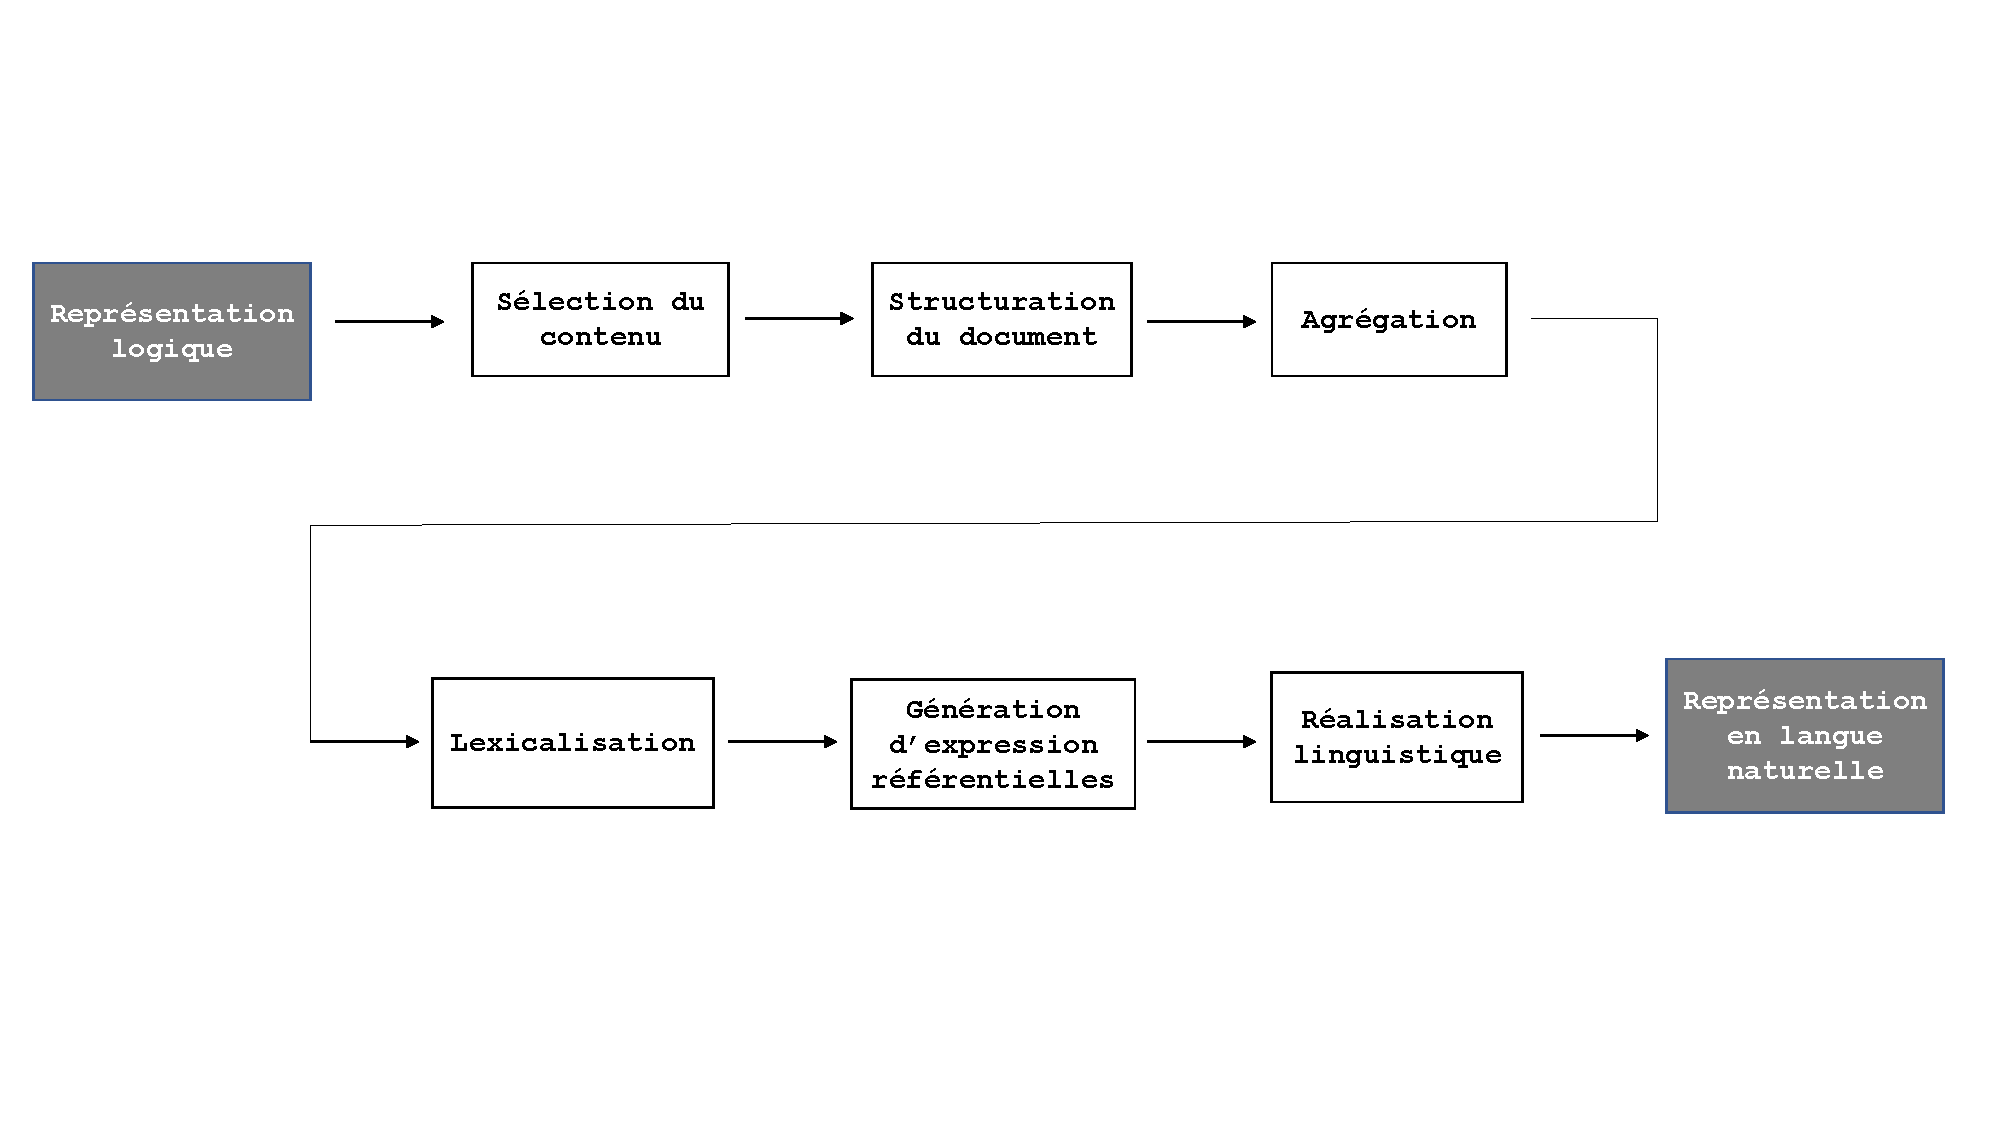
\includegraphics[width=1\textwidth, trim = {0cm 0cm 0cm 0cm},clip]{ch2/figs/pipeline.pdf}
	\caption{Pipeline classique}
	\label{fig:Pipeline}
\end{figure}

Beaucoup s'entendent pour dire qu'il y a deux section : le quoi-dire et le comment-le-dire (Danlos, 1983) et \citep{GattSurveyStateArt2017} qui l'appelle le early process et le late process. Les deux renvoient aux mêmes concepts. Cette distincion implique nécessairement un ordre dans le temps dans lequel les tâches seront exécutées, pour les systèmes modulaires. Toutefois, cet ordre est remis en question dans les dernières années \citep{GattSurveyStateArt2017}.

\subsection{Sélection du contenu}

Un système NLG doit décider quelle information sera inclue dans le texte en construction et quelle information ne devrait pas y être. La sélection du texte dépend entre autre de l'objectif de la tâche (par exemple si un texte est adressé à un débutant ou un expert), ainsi typiquement , il y a plus d'information ou de détails dans les données que d'information que nous voulons transmettre en texte. Ainsi, la sélection de contenu implique des choix. Par exemple, s'il s'agit de données pour un match de soccer, on ne voudrait probablement pas réaliser toutes les passes et les fautes commises durant le match, bien que ces informations figurent dans les données en input. Il faut donc les filtrer et créer des représentations sémantiques de l'information qui sont souvent exprimé en représentation formelle du langage comme des représentations logiques, des base de données, des matrices ou des graphes.

\subsection{Structuration du document}
Après avoir sélectionné le contenu, un système NLG doit décider l'ordre dans lequel les informations seront présentées. Par exemple, si on utilise encore l'exemple du soccer, on commencerait par les informations générales liées au match (où et quand le match a eu lieu, entre quelles équipes, qui était blessé cette journée, etc), puis la description des buts comptés en ordre chronologique. Ce qui résulte de cette étape du processus est le plan d'un texte : une représentation ordonnée et structurée de messages à transmettre. Durant les dernières années, il y a eu des tentatives d'implémenter des méthodes d'apprentissage machine pour que la structuration de document se fasse automatiquement (Dimitromanolaki et Androutsopoulos,2003; Althaus et al., 2004)

\subsection{Agrégation}
Ce ne sont pas tous les messages sélectionnés dans le plan qui doivent être exprimés dans des phrases individuelles. En combinant des phrases individuelles en une seule et même phrase, on génère un texte beaucoup plus fluide et agréable à lire (Cheng et Mellish, 2000). Ainsi, la majeure partie du temps, elle sert à enlever la redondance dans le texte. Encore une fois, des chercheurs tentent d'automatiser cette étape en implémentant des méthodes d'apprentissage machine pour que le système NLG apprenne les règles d'agrégation et les applique lorsqu'il se doit (Barzilay et Lapata, 2006).

\subsection{Lexicalisation}
À cette étape, nous avons des données sélectionnées, puis structurées et que les futures phrases ont été combinées, on peut commencer à traduire les données en langue naturelle. Cette partie est très importante car c'est là qu'on choisi les mots qui seront utilisés pour transmettre le message. Toutefois, cette section se complique parfois car il existe naturellement plusieurs manières différentes de dire la même chose. La complexité de ce processus de lexicalisation dépend des mécanismes intégrés au système pour gérer cela. Certains traitent de lexicalisation en surface, d'autres la traite profondément. Toutefois, ceux qui traitent la lexicalisation en surface sont beaucoup plus restreints dans leur choix et sont très rigides. Tandis qu'un modèle profond permet de mieux tenir compte de la richesse lexicale d'une langue, mais il faudra une approche qui unit les représentations conceptuelles avec des règles de grammaire qui encoderont les choix lexicaux et syntaxiques. D'ailleurs, Elhadad et al. 1997 avait grandement contribué pour cela.

Convertir un graphe sémantique d'entités et de relations, en un graphe syntaxique de mots et de relations syntaxiques. 

\subsection{Génération d'expressions réferentielles}
Souvent référée comme étape discriminatoire dont le but est de déterminer quelles informations doivent être générées pour qu'on puisse distinguer toutes les entités en jeu. Le but est de s'assurer que le lecteur peut idientifier chaque entité dans le texte. La meilleure manière de référer à une entité donnée.
Il s'agit de la tâche pour sélectionner des mots ou des phrases qui identifieront des entités. C'est une étape du processus qui a reçu beaucoup d'attention, car il n'y a toujours pas de consensus quant à la manière de faire et c'est extrêmement difficle. (Compléter avec les autres articles)

\subsection{Réalisation linguistique}
La dernière étape de ce pipeline NLG classique est la réalisation linguistique. Lorsque tous les mots, puis successivement les phrases ont été choisies, il faut les combiner en des phrases grammaticales. 

Cette tâche implique la morphologie et la linéarisation. De même qu'insérer les mots fonctionnels (auxiliaires, etc.) et la ponctuation.

\subsubsection{À base de patrons}
Est utilisé lorsque le domaine est petit et que les variations sont minimes. (McRoy et al., 2003). Montrer un exemple avec le soccer. (p.19).  L'avantage d'utiliser les templates est qu'on peut très bien prévoir ce qui sera généré en output, donc les risques d'erreurs grammaticales sont extrêmement faibles, du au contrôle qu'on a. Ils peuvent aussi être complémenter par des modules de règles pour pallier à certains problèmes, ce qui les rend très performant. Toutefois, l'inconvénient de tels systèmes est qu'ils sont très coûteux en termes de temps, puisque tout doit être fait à la main. Bien qu'avec la mode de l'apprentissage machine, certains systèmes apprennent à écrire des patrons (Angeli et al., 2012). Finalement, ils ne fonctionnent pas bien avec des tâches qui requièrent beaucoup de variation linguistique.

\subsubsection{À base de règles grammaticales}


\subsubsection{Statistique}

\subsubsection{Règles vs statistiques : avantages/inconvénients}
(Belz et Kow, 2009)


\subsection{NLG architecture et approches}

Manières différentes d'opérer ces tâche

\subsubsection{modulaire}
\subsubsection{planifiée}
\subsubsection{globale}

\section{Réalisateurs}

Nous parlerons plus précismént de différents réalisateurs, car notre travail repose sur le perfectionnement d'un réalisateur. 

\subsection{Surge}

\subsection{KPML}

\subsection{RealPro}

\subsection{SimpleNLG}

\subsection{MARQUIS}
\subsubsection{MATE}
utilise aussi la TST

\subsection{Forge: héritier de MARQUIS}

\subsection{GenDR : héritier de MARQUIS}
utilise aussi MATE
Un réaliseur linguistique
\subsubsection{Lexicalisation}
\subsubsection{Arborisation}

\section{Dictionnaire et les verbes dans les réalisateurs : pour les rule-based system}
mentionner les dictionnaires qui disent que les verbes sont les plus importants
Expliquer c'est quoi un patron de régime/cadre de sous-catégorisation, valence, etc.
permettent de couvrir large
patrons de régime des verbes y sont encodés
